\documentclass[tikz]{standalone}
\usetikzlibrary{calc}

\begin{document}

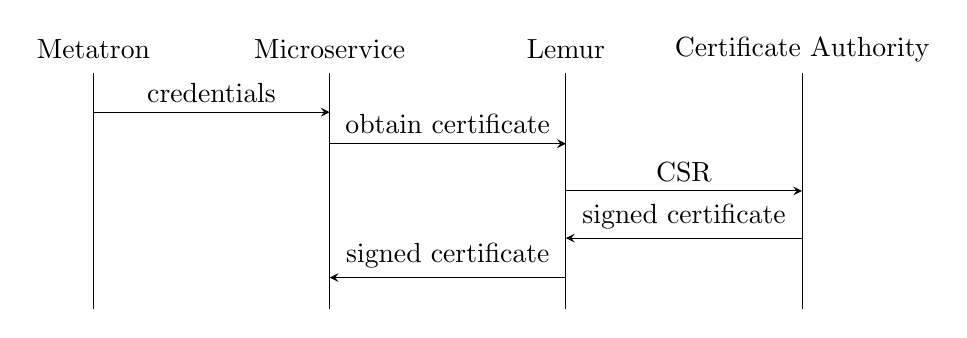
\begin{tikzpicture}
	\draw (-3,0) -- (-3,-3);
	\draw (0,0) -- (0,-3);
	\draw (3,0) -- (3,-3);
	\draw (6,0) -- (6,-3);
	\node (metatron) at (-3,.3) {Metatron};
	\node (microservice) at (0,.3) {Microservice};
	\node (lemur) at (3,.3) {Lemur};
	\node (ca) at (6,.3) {Certificate Authority};

	\draw[-stealth] (-3, -0.5) -- node[midway, above] {credentials} (0, -0.5);
	\draw[-stealth] (0, -0.9) -- node[midway, above] {obtain certificate} (3, -0.9);
	\draw[-stealth] (3, -1.5) -- node[midway, above] {CSR} (6, -1.5);
	\draw[-stealth] (6, -2.1) -- node[midway, above] {signed certificate} (3, -2.1);
	\draw[-stealth] (3, -2.6) -- node[midway, above] {signed certificate} (0, -2.6);
	%\draw[-stealth] (0, -2.1) -- node[pos = .35, above left] {signed certificate} (6, -2.1);
	%\node[above,font=\large\bfseries] at (current bounding box.north) {Use same JWT for each request};
\end{tikzpicture}

\end{document}

